%%%%%%%%%%%%%%%%%%%%%%%%%%%%%%%%%%%%%%%%%%%%%%%%%%%%%%%%%%%%%%%%%%%%%%%%%%%%%%%%
%2345678901234567890123456789012345678901234567890123456789012345678901234567890
%        1         2         3         4         5         6         7         8

\documentclass[letterpaper, 10 pt, conference]{ieeeconf}  % Comment this line out if you need a4paper

% \documentclass[letterpaper, 12 pt, twoside]{report}  % Comment this line out if you need a4paper


%\documentclass[a4paper, 10pt, conference]{ieeeconf} % Use this line for a4 paper

% \IEEEoverridecommandlockouts %This command is only needed if you want to use the \thanks command

\overrideIEEEmargins  % Needed to meet printer requirements.

%In case you encounter the following error:
%Error 1010 The PDF file may be corrupt (unable to open PDF file) OR
%Error 1000 An error occurred while parsing a contents stream. Unable to analyze the PDF file.
%This is a known problem with pdfLaTeX conversion filter. The file cannot be opened with acrobat reader
%Please use one of the alternatives below to circumvent this error by uncommenting one or the other
%\pdfobjcompresslevel=0
%\pdfminorversion=4

% See the \addtolength command later in the file to balance the column lengths
% on the last page of the document

% The following packages can be found on http:\\www.ctan.org
\usepackage{graphicx} % for pdf, bitmapped graphics files
%\usepackage{epsfig} % for postscript graphics files
%\usepackage{mathptmx} % assumes new font selection scheme installed
%\usepackage{times} % assumes new font selection scheme installed
\usepackage{amsmath} % assumes amsmath package installed
\usepackage{amssymb}  % assumes amsmath package installed
%\usepackage{dsfont}
\usepackage{algorithm}
\usepackage{algorithmic}
\usepackage{commath}

\usepackage{xcolor}
\newcommand{\todo}[1]{{\color{blue}[TODO: #1]}}
\newcommand{\response}[1]{{\color{green}[RESPONSE: #1]}}
\graphicspath{{figures/}}


\DeclareMathOperator*{\argmax}{arg\,max}
\DeclareMathOperator*{\argmin}{arg\,min}

\title{\LARGE \bf
Multi-Agent Autonomous Mapping of Unknown GPS-Denied Environments Using a Relative Navigation Framework}

\author{Jacob M. Olson$^{1}$, Timothy W. McLain$^{2}$% <-this % stops a space
\thanks{Thanks to Mathieu Labbe for being responsive to answering questions on the RTAB-Map forum and helping with developing the map merging node.}% <-this % stops a space
\thanks{$^{1}$The corresponding author can be contacted at
        {\tt\small jacobmo at byu.edu}.}%
\thanks{$^{2}$All authors are with the Department of Mechanical Engineering or Electrical and Computer Engineering,
        Brigham Young University, Provo, UT, 84602, USA.}%
%\thanks{$^{3}$C. Peterson is with the Faculty of Electrical and Computer Engineering,
%		Brigham Young University, Provo, UT, 84602, USA.
%        {\tt\small cammy.peterson at byu.edu}}%
%\thanks{$^{4}$R. W. Beard is with the Faculty of Electrical and Computer Engineering,
%		Brigham Young University, Provo, UT, 84602, USA.
%        {\tt\small beard at byu.edu}}%
}

\begin{document}

\maketitle
\thispagestyle{empty}
\pagestyle{empty}


%%%%%%%%%%%%%%%%%%%%%%%%%%%%%%%%%%%%%%%%%%%%%%%%%%%%%%%%%%%%%%%%%%%%%%%%%%%%%%%%
\begin{abstract}

\todo{write the abstract}

\end{abstract}


%%%%%%%%%%%%%%%%%%%%%%%%%%%%%%%%%%%%%%%%%%%%%%%%%%%%%%%%%%%%%%%%%%%%%%%%%%%%%%%%
\section{Introduction}

\todo{write the rest of the introduction (mapping/slam background)}
Mapping an environment where GPS (global positioning system) signals are degraded or entirely unavailable such as an earthquake damaged building is not a trivial task. Many common mapping approaches rely on high quality GPS data in order to patch together data to generate a map \todo{throw a citation or two here that need GPS}. Often these GPS-denied environments are inaccessible to ground robots due to difficult terrain, especially in locations like earthquake damaged buildings. This necessitates the use of UAVs (unmanned aerial vehicles) to carry out some or all of the mapping. Because of the limited flight time of UAVs, the mapping process can be streamlined by using multiple UAVs collaborating to build a map.

\todo{cite the ground and air paper, talk about simultaneous mapping, is this much background appropriate for a paper? }


The remainder of the paper is organized as follows: Section \ref{approach} describes the framework used to map the environment, and background on what previous work has made this research possible. Section \ref{planning} details the planning and control schemes used to successfully navigate the unknown area. The method used to combine maps of multiple agents is then explained in Section \ref{merge}. Results showing and evaluating the generated maps are presented in Section \ref{results}. Finally, conclusions are presented in Section \ref{conclusions}.

%%%%%%%%%%%%%%%%%%%%%%%%%%%%%%%%%%%%%%%%%%%%%%%%%%%%%%%%%%%%%%%%%%%%%%%%%%%%%%%%
\section{Technical Approach}\label{approach}

\subsection{Problem Statement}

The goal of this paper is to show how to successfully map a GPS-denied environment using multiple UAVs collaborating with each other. For map building to be successful, a flight path that produces high quality loop closures and good coverage of its environment is required. This paper does not focus on how to plan these high level paths. The framework presented in this section assumes that a high quality path will be supplied either by the user or by a high-level coverage path planner. The focus of this paper is first, to show that properly estimating UAV states allows for successful GPS-denied navigation, and secondly, how to extend streamline the mapping process by merging maps of several UAVs into a single map. A high-level network diagram is shown in Fig. \ref{fig:rtab_network} which outlines the framework used in this paper to successfully generate a single merged map from multiple UAVs in a GPS denied environment. Each section of the diagram will be described in detail throughout the paper.

\begin{figure*}
\centering
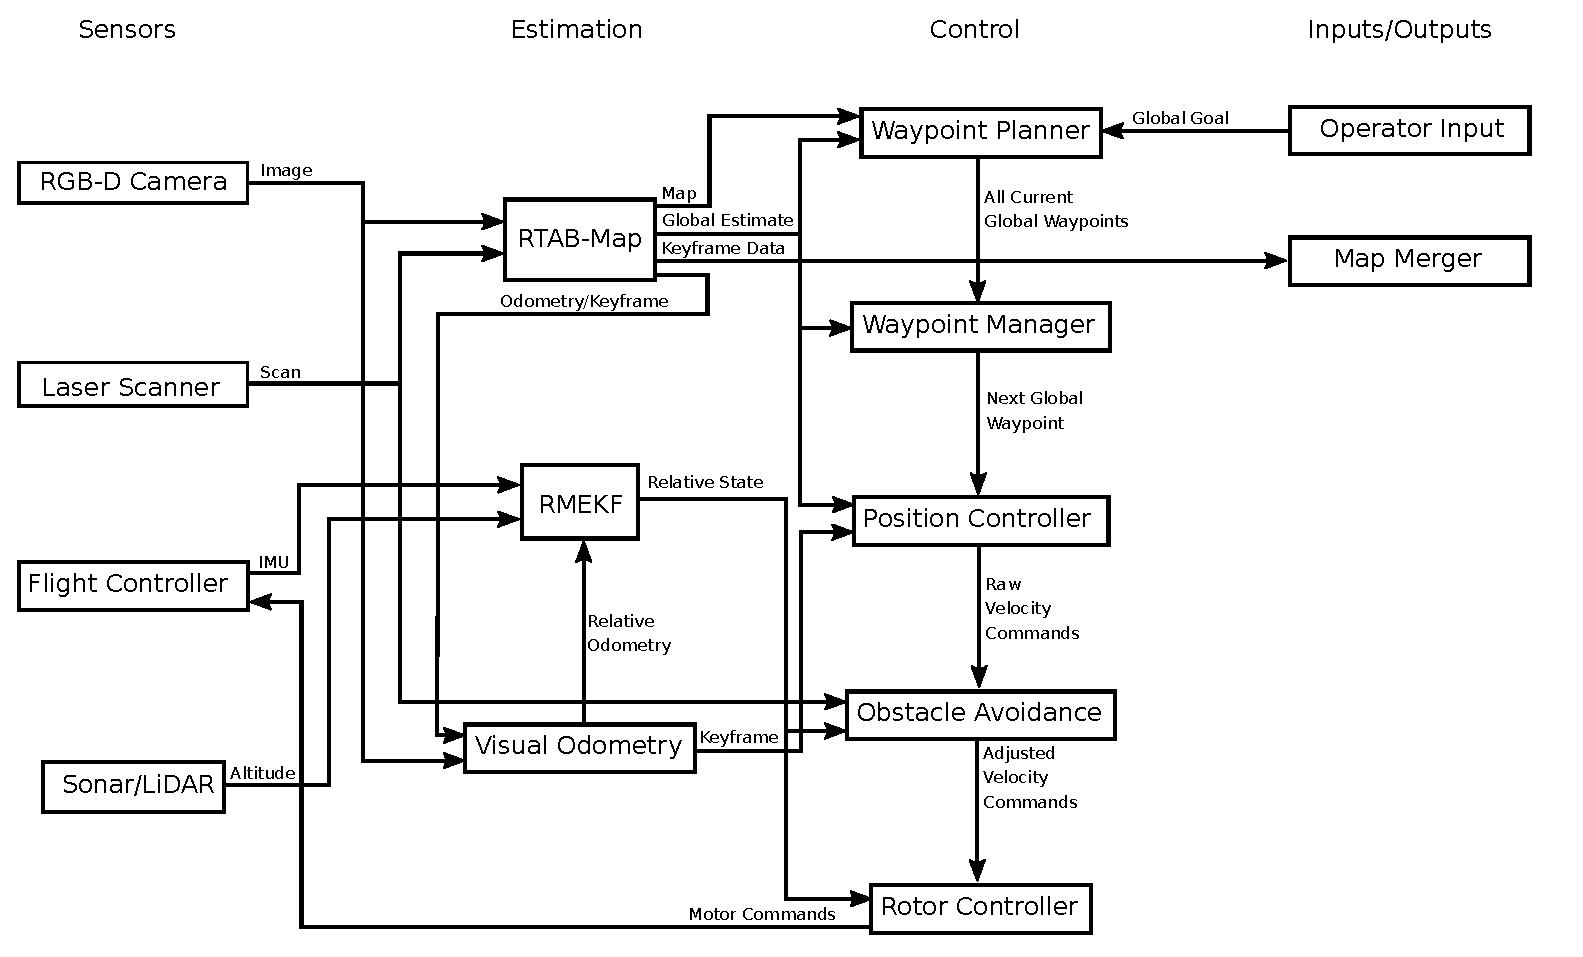
\includegraphics[width=1.0\linewidth]{rtab_relative_nav_network}
\caption{The network diagram of the relative navigation framework proposed in this paper}
\label{fig:rtab_network}
\end{figure*}

\subsection{Sensors}

Since we are operating in a GPS-denied environment, we are not able to rely on GPS measurements to give us global information about where the UAVs are located. As shown in Fig. \ref{fig:rtab_network} the sensors used by the UAV to estimate its state are an RGB-D camera, a planar LiDAR laser scanner, a single-beam LiDAR range finder and an IMU on the onboard flight controller. Using only these sensors and the flight computer, we must be able to accurately estimate the states of the UAV enough to send waypoints and control the attitude. We talk about how these sensors are used to accurately estimate the UAV's state in the next section. \todo{how much do I talk about sensors here?}

\subsection{Estimation}

Estimation is the most critical element in enabling autonomous flight. Without good position and attitude estimation, autonomous navigation algorithms cease to function. We use a graph-SLAM approach based from that presented by Thrun et al. \cite{Thrun2006} to navigate and generate the maps. when using a graph based SLAM approach, loop closures can cause problems with the estimation if it not done correctly. Every time the UAV sees the same objects from a similar location as before, a new loop closure is detected and the map and position estimate are re-optimized. If the new loop closure results in a large shift in the current position estimate, a naive estimator can diverge because the new position lies outside of the covariance bounds. To avoid the issue of loop closures causing instability in the controller, we estimate the global and relative states of the UAV separately and do not rely on the global state estimate to control the attitude of the UAV.

The current global state estimates are stored in a transformation tree as shown in Fig. \ref{fig:tf_tree}. The $\mathit{world}$ frame is the inertial NED (North, East, Down) frame of the world with a static origin. The UAV's starting location with respect to the world is set as a static transform between the $\mathit{world}$ and $\mathit{map}$ frames with a rotation into the inertial NWU (North, West, Up) orientation. The $\mathit{base\_link}$ transform represents the current estimated position of the the UAV in the NED orientation and $\mathit{camera\_link}$ represents the position in the NWU orientation, the $\mathit{camera\_base\_link}$ transform represents the current position of the camera in the camera frame.

The $\mathit{odom}$ frame is used to adjust for loop closures. When the flight begins, the $\mathit{odom}$ frame starts with zero transformation from the $\mathit{odom}$ frame. Every time a loop closure is detected and the map is re-optimized, the transform between the $\mathit{map}$ and $\mathit{odom}$ frames is adjusted to reflect the correction. This way the transform between the $\mathit{odom}$ frame and the robot frame $\mathit{camera\_link}$ and $\mathit{base\_link}$ stays continuous when loop closures are detected even though the position estimate is not.

The $\mathit{keyframe}$, $\mathit{keyframe\_world}$ and $\mathit{keyframe_camera}$ frames are used for computing the relative visual odometry used for the relative estimation. The transform between the $\mathit{keyframe}$ and $\mathit{camera\_link}$ frames is used as the relative odometry in the estimator.

The current waypoint that the UAV is flying towards is represented as the transform between the $\mathit{world}$ and $\mathit{waypoint}$ frames. This way a loop closure does not shift the desired global position of the waypoint. The position controller drives the transform between the $\mathit{waypoint}$ and $\mathit{base\_link}$ frames to zero.

More detail regarding the uses and implementations of these transforms will be further explained in the following sections.

%This is under the assumption that the desired waypoint location is known globaly, this could be modified to set the new waypoint relative to odom frame if the position is relative to the current obstacles rather than the global position.

\begin{figure*}
\centering
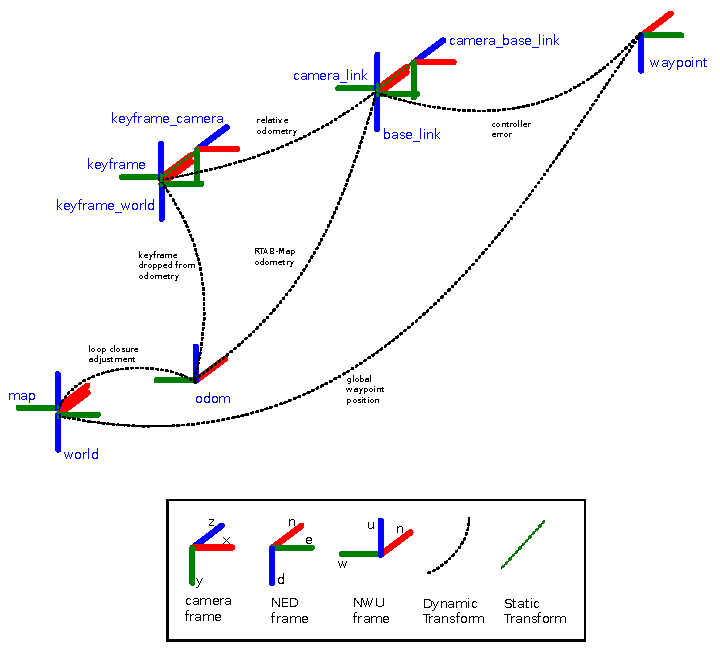
\includegraphics[width=0.9\linewidth]{tf_tree_relative_rtab}
\caption{The transformation tree of the reference frames used in estimation and control.}
\label{fig:tf_tree}
\end{figure*}

\subsubsection{RTAB-Map}

RTAB-Map (real-time appearence-based Mapping), developed by Labbe et al. \cite{Labbe2011}\cite{Labbe2013}\cite{Labbe2019}, is a powerful open source software package that uses graph-based SLAM with appearance-based loop closures to generate high-quality, dense 3D maps of environments without the use of GPS.  RTAB-Map is also able to accurately estimate the UAV position within the map with little error. We use the RGBD-Odometry visual odometry from RTAB-Map as detailed in \cite{Labbe2019} as an input to the estimation for the relative framework.

The current functionality of RTAB-Map does not allow for multiple agents mapping simultaneously to combine the maps into a single one. This paper proposes a method to extend the functionality of RTAB-Map to combine the maps of multiple agents flying simultaneously into a single map in near real time. The implementation of this method is detailed in section \ref{merge}.

RTAB-Map manages the $\mathit{map}$, $\mathit{odom}$, $\mathit{base\_link}$, $\mathit{camera\_link}$, and $\mathit{camera\_base\_link}$ frames used in the tf tree and their respective transforms.

We use the current global estimate of RTAB-Map for the position controller and waypoint manager. But because of the inevitable inaccuracies and the lower estimate rates of RTAB-Map, we do not use global estimates to do attitude control on the UAVs. Rather, we use a relative navigation framework to estimate the attitude and relative state.

\subsubsection{Visual Odometry}

The odometry and keyframe information generated by RTAB-Map is used to generate a relative odometry message that is used by the relative estimator. RTAB-Map produces a global visual odometry which provides a real time estimate of the global position and orientation of the UAV. As new keyframes in the odometry are declared and new nodes are added to the graph, the visual odometry node shown in Fig \ref{fig:rtab_network} resets the transform between the $\mathit{keyframe}$ and $\mathit{camera\_link}$ frames to zero. As previously mentioned, the relative odometry used in the estimator comes from the transform between the $\mathit{keyframe}$ and $\mathit{camera\_link}$ frames. Because of the constant resetting of the keyframe transform, the odometry used by the relative estimator is much less susceptible to drift over time. because it is only tracking the transform between keyframes.

\subsubsection{RMEKF}

The Relative Multiplicative Extended Kalman Filter (RMEKF) which is the heart of the relative navigation framework established by Wheeler et al. \cite{Wheeler2017}\cite{Wheeler2018} and Koch et al. \cite{Koch2017} was shown to successfully estimate the UAV's relative state sufficient to autonomously navigate in GPS-denied environments that had been previously mapped. Thus far, however, it has not been extended to estimation and navigation in unknown and unmapped environments, this paper proposes a method to extend the functionality to these environments.

The RMEKF takes as inputs the IMU measurement from the flight controller, the relative visual odometry from keyframes as previously described, and the attitude measurement from the LiDAR single beam range finder. Then using the multirotor dynamics model, is able to accurately estimate the relative state of the UAV which is used for obstacle avoidance and high rate attitude control. It is important to note that the RMEKF makes no effort to estimate the global position of the UAV. This makes it so that large corrections in the estimated global position that happen with loop closures do not cause the estimator to diverge, and therefore cause stability issues in the velocity and attitude controllers onboard the UAV. The RMEKF functionality and results are further detailed in \cite{Koch2017}.

\subsection{Control}

To successfully control a UAV in a GPS-denied environment, the control must be segmented into different categories to take advantage of both global and relative estimates. The control scheme, as shown inf Fig. \ref{fig:rtab_network}, cascades beginning with inputs of the current obstacle map, estimated position, and goal position and ending with outputting the motor commands to the flight controller.

\subsubsection{Waypoint Planner}

The first stage of the control is the waypoint planner. Its inputs are the global goal, current known obstacles, and current global estimates and it outputs a path to the goal that avoids all known obstacles as set of waypoints. This stage will be further explained in Section \ref{planning}.

\subsubsection{Waypoint Manager}

After receiving the current set of waypoints, the waypoint manager selects the appropriate waypoint for the UAV to fly towards and sends the global location to the position controller. The waypoint manager monitors the position and heading error between the current estimated position and the current waypoint and when the error crosses below a user-defined threshold value, the next waypoint is sent to the position controller.

\subsubsection{Position Controller}

The position controller uses the error between the current estimated position and heading of the UAV and the next waypoint. The goal of the position controller is to drive the error to zero. Since it operates in the error space of the the UAV rather than the state space, sudden shifts in the UAVs position estimate caused by loop closures have minimal effect on the controller and it is able to continue controlling the error to zero. The output of the position controller is a velocity command for the UAV.

\subsubsection{Obstacle Avoidance} \label{obs_avoid}

Before passing the velocity control into the attitude controller, it is filtered through an obstacle avoidance node as described by Jackson et al. \cite{Jackson2016}. This node uses the current relative estimates and obstacles detected by the planar laser scanner and using cushioned extended-periphery avoidance (CEPA), it pushes away from obstacles and towards the current waypoint. The obstacle avoidance node then sends the modified velocity command to the attitude controller.

\subsubsection{Attitude Controller}

The attitude controller is a conventional PID controller that takes the velocity input commands and outputs the motor commands to the flight controller.

\subsection{Inputs/Outputs}

The input for each agent in the system is the desired goal location either from operator input or from a high level path planner. As each agent flies through the environment and builds their own maps, at each keyframe, they send the keyframe data consisting of the color and depth images and features from the images to the map merger where the maps are combined into a single node. The map merger will be further explored in Section \ref{merge}.

%%%%%%%%%%%%%%%%%%%%%%%%%%%%%%%%%%%%%%%%%%%%%%%%%%%%%%%%%%%%%%%%%%%%%%%%%%%%%%%%
\section{Planning}\label{planning}

The reactive planner we use is a form of rapidly-exploring random trees (RRT) planner like that originally developed by Lavalle et al. \cite{Lavalle1998} with a path smoothing approach similar to that proposed by Beard and McLain \cite{Beard2012}. RRT path planning is very effective for planning in real time with dynamic obstacles because it randomly searches the full, non-discretized environment for feasible paths rather than using an exhaustive search and needing to discretize the environment like many other planners require. Because the planner uses a dense 2D grid map of all currently known obstacles, some adjustments were made for it to efficiently plan and check for obstacles, and re-plan when new obstacles were discovered in the current path.

\subsection{Global Goal Following with Relative Estimation}

As mentioned earlier, the relative estimation that is critical to keeping the UAV airborne makes no attempt to estimate the global position of the UAV, but only its relative state with respect to the last keyframe. By doing so, the global estimate of the position does not have to be continuous and is able to slide and adjust with loop closure corrections without affecting the estimator. The path planner uses RRT to plan a global path from the current position to the goal. Because these global paths do not adjust with loop closures, and because the map is being made as the UAV flies, it is necessary for the planner to be able to dynamically re-plan as the map adjusts for loop closures and new obstacles are added to it.

\subsection{Reactive Path Planning}

Fig. \ref{fig:reactive_plan} shows the process of the is dynamic path planning. When the UAV starts, it knows very little about the environment. The only obstacles that it knows about are the ones that are within line-of-sight of the laser scanner when it begins. The UAV plans a path to the current goal which avoids the obstacles that it can initially see. As it flies, the obstacle map is continuously updated with new obstacles. Each time the map updates, the current flight path is checked for collisions with any obstacles. If collisions are found, a new path is planned to the goal from the current location to avoid the newly discovered obstacles. This process continues until the agent is able to successfully reach the goal. Since the path is updated any time an obstacle is detected in its path, no prior knowledge of the environment is required to begin flying.

\begin{figure*}
\centering
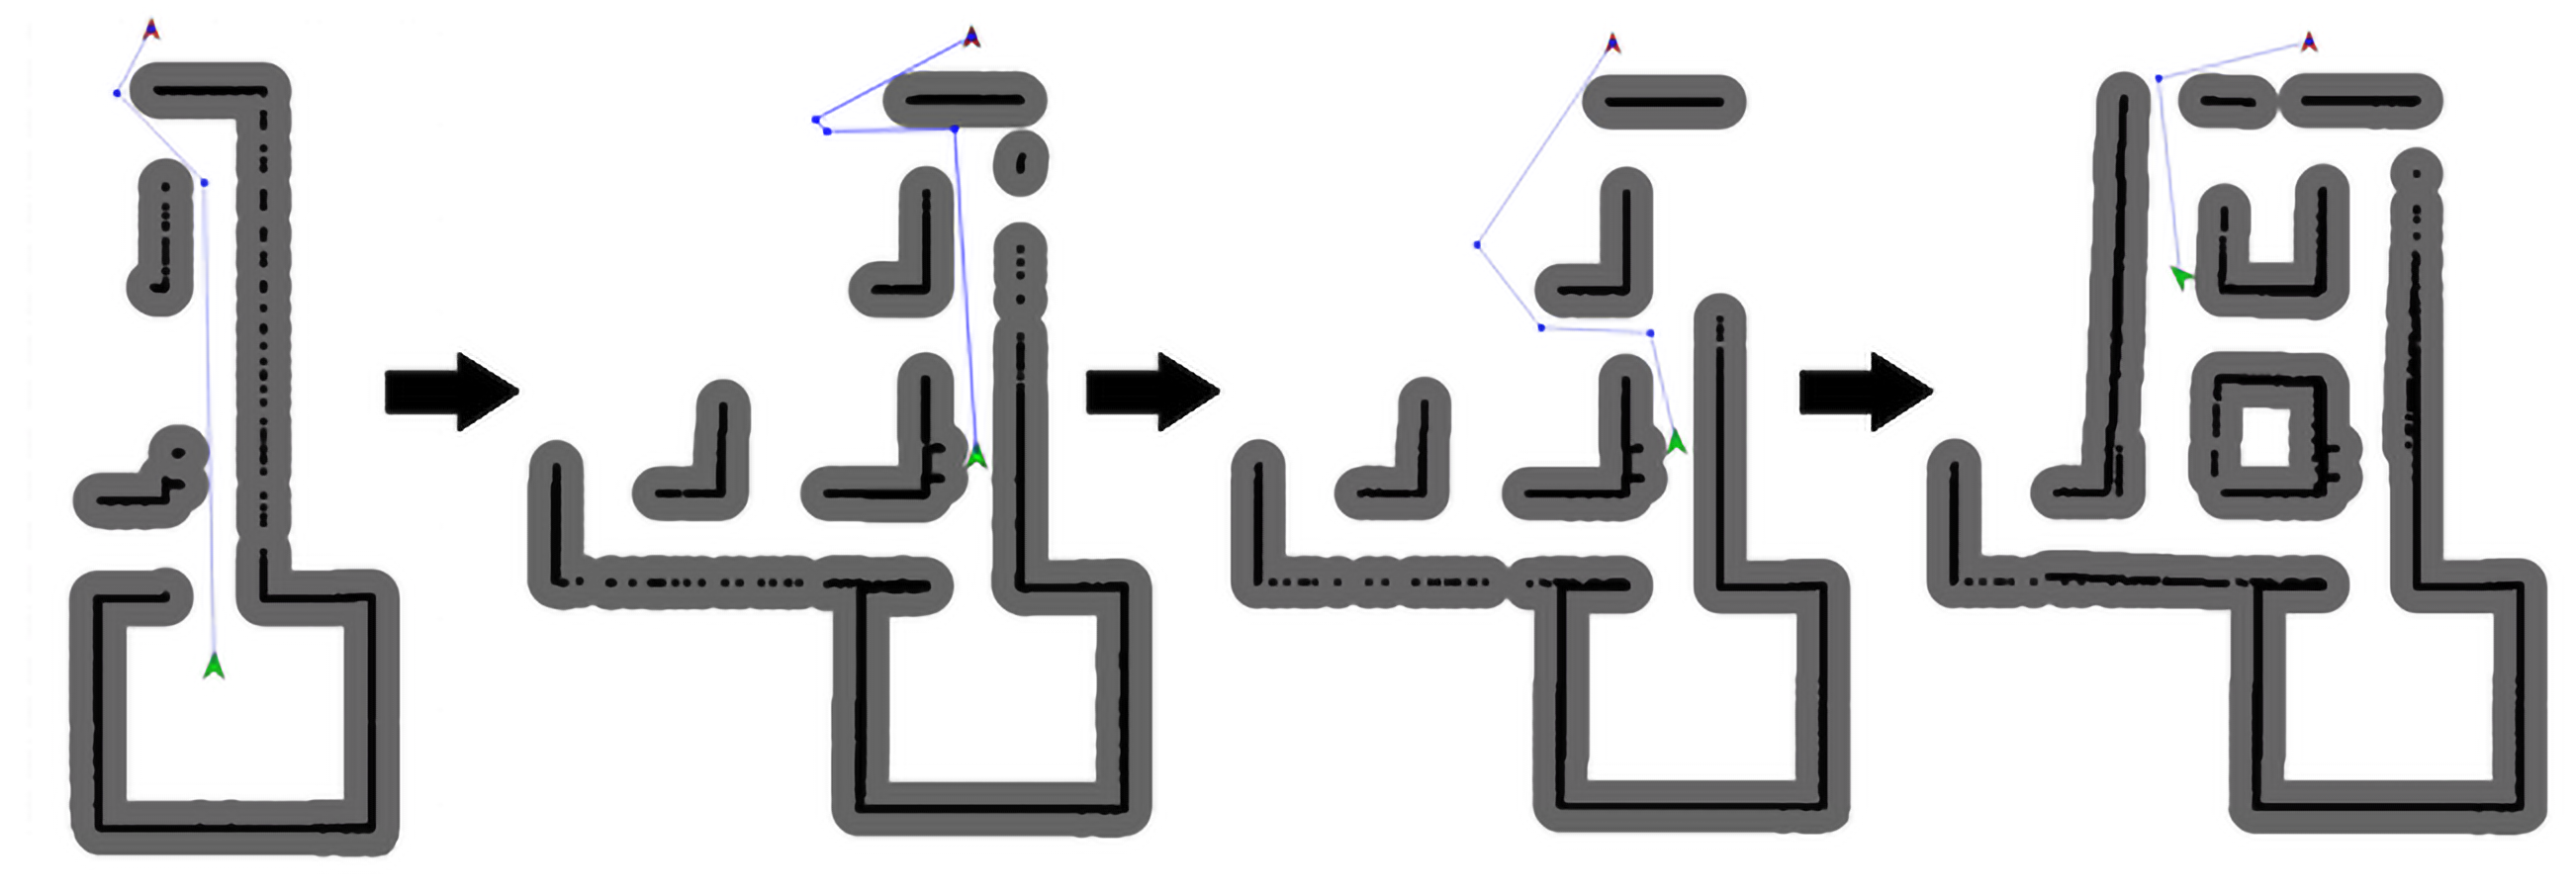
\includegraphics[width=1.0\linewidth]{adaptive_path_plan2.png}
\caption{An example of how the reactive path planner works as the UAV flies the planned path. The current estimated position is marked by the green arrow, the current goal position is marked by the red arrow, and the current path planned is marked with the blue lines. Detected obstacles with their respective safety buffers are represented with black and grey respectively.}
\label{fig:reactive_plan}
\end{figure*}

Since this planner is used in conjunction with the CEPA obstacle avoidance node explained in \ref{obs_avoid}, the UAV is able to effectively avoid obstacles in emergency situations at a much higher rate than the planner runs. It is also able to navigate through complex maps that would not be possible with only obstacle avoidance. As long a possible path to the goal exists, the RRT planning will find a way to reach the goal. as mentioned before, in most cases it will find a path to the goal in far less time than an exhaustive search method would. More recently, new improvements to RRT have been explored such as RRT* developed by Karaman et al. \cite{Karaman2011} which is able to guarantee asymptotically optimal paths. Since this planner is used as a form of exploration of unknown environments however, we decided to not extend the planner to use RRT* to allow it to be more random in the flight path to encourage more exploration of the map while flying paths.

\subsubsection{Efficient Collision Detection}
Most implementations of RRT have few large obstacles that are planned around but the obstacles we use are from 2D grid map generated by the current map in RTAB-Map. So rather than having just a few large obstacles, there are many small obstacles. So using a standard obstacle detection check with each propagation of the RRT would be extremely inefficient. To maximize the efficiency during planning, only obstacles within range of the candidate node and its connection to the tree are checked. An example of how this works is illustrated in Fig. \ref{fig:rrt_sample}.

\begin{figure}
\centering
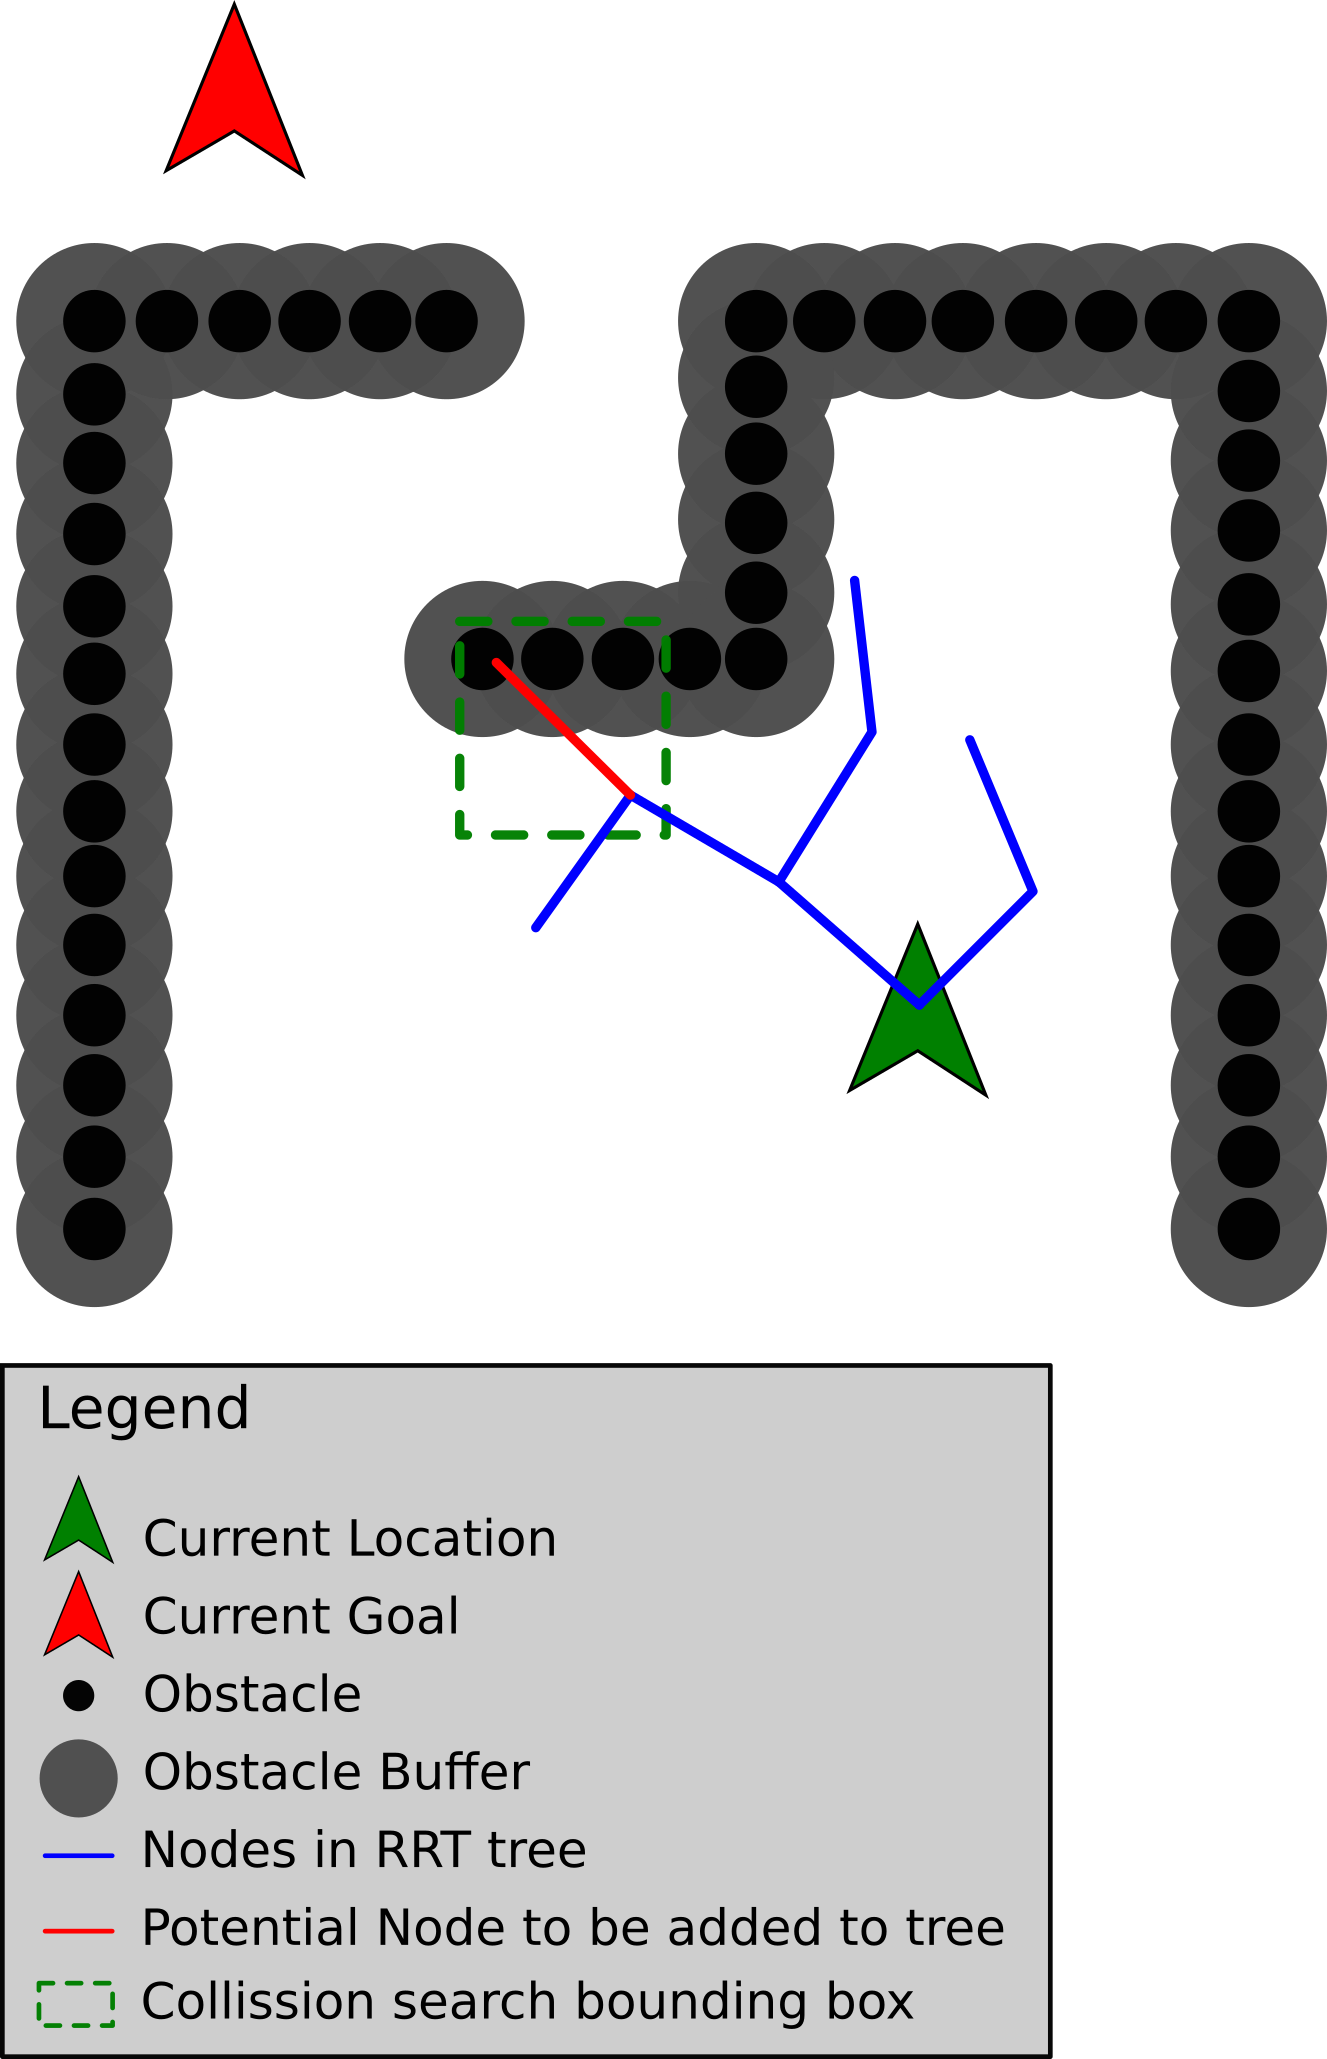
\includegraphics[width=0.8\linewidth]{rrt_sample}
\caption{Example of one step of collision check with the RRT planner.}
\label{fig:rrt_sample}
\end{figure}

As the RRT tree propagates, before each candidate node is added to the tree, an obstacle collision check is done on the obstacles within range of the new node. The obstacles are determined to be in range if they are either between both x and y locations of the line formed connecting the candidate node to the tree or within one buffer radius of those points. The green bounding box in Fig. \ref{fig:rrt_sample} shows which obstacles would be included in this obstacle check. To check the if the obstacles would collide, we check to see if their perpendicular distance to the line is less than the buffer radius. With the following equations.

\begin{align}
  d &= \dfrac{|\Delta y*x_{\mathit{obs}} -
      \Delta x*y_{\mathit{obs}} + \Delta s|}
      {\sqrt{\Delta y^2 + \Delta x^2}}\\
  \nonumber \text{with}\\
  \Delta x &= x_2 - x_1\\
  \Delta y &= y_2 - y_1\\
  \Delta s &= x_2*y_1 -x_1*y_2
\end{align}

$(x_1,y_1)$ and $(x_2,y_2)$ are the endpoints of the candidate node line and $(x_{\mathit{obs}},y_{\mathit{obs}})$ is the location of the obstacle being checked. If the distance $d$ is less than the buffer radius, a collision is detected and the candidate is rejected. By only checking for collisions with obstacles within the bounding box, nearly all obstacles are ignored in most cases. This significantly improves performance of the RRT planner and allows it to plan in real time and dynamically update the path whenever needed. The collision detection for path smoothing and path checking works the same way, with $(x_1,y_1)$ and $(x_2,y_2)$ being the endpoints of each path segment.

% \subsection{Path Planning Algorithm}
% The path planning breaks down to four separate functions. The RRT planner, collision checker, path smoother, and path checker. Each time the obstacles are updated, the path checker is run to see if the current path is still valid. If invalid, the RRT planner is run from the current location then the path is smoothed following the
%
%
% \begin{algorithm}
%   \caption{Dynamic Path Planner}
%   \label{dyn_path_plan}
% \begin{algorithmic}
%     \IF{some condition is true}
%         \STATE do some processing
%     \ELSIF{some other condition is true}
%         \STATE do some different processing
%     \ELSE
%         \STATE do the default actions
%     \ENDIF
% \end{algorithmic}
% \end{algorithm}
%
%
% \todo{include algorithm section to explain what the planner is doing? or just more explanation? or is this good enough?}

%%%%%%%%%%%%%%%%%%%%%%%%%%%%%%%%%%%%%%%%%%%%%%%%%%%%%%%%%%%%%%%%%%%%%%%%%%%%%%%%
\section{Map Merging}\label{merge}

The map merging process proposed in this paper is able to generate a combined map from multiple agents on a base station computer in near real time while the UAVs are still simultaneously mapping the environment.

Fig. \ref{fig:map_merge} shows the network diagram of the process of merging the maps. To merge the maps in near real time, each time a new keyframe is initialized, the data from the keyframe consisting of the color and depth information from the keyframe, and the features extracted from the color image are stored in a database referred to as RGB-D Cache which is hosted on the base station computer. A 3D XYZRGB pointcloud is generated using the color and depth images from the RGB-D camera onboard and the features are generated from either SIFT/SURF or ORB using OpenCV.

\begin{figure*}
\centering
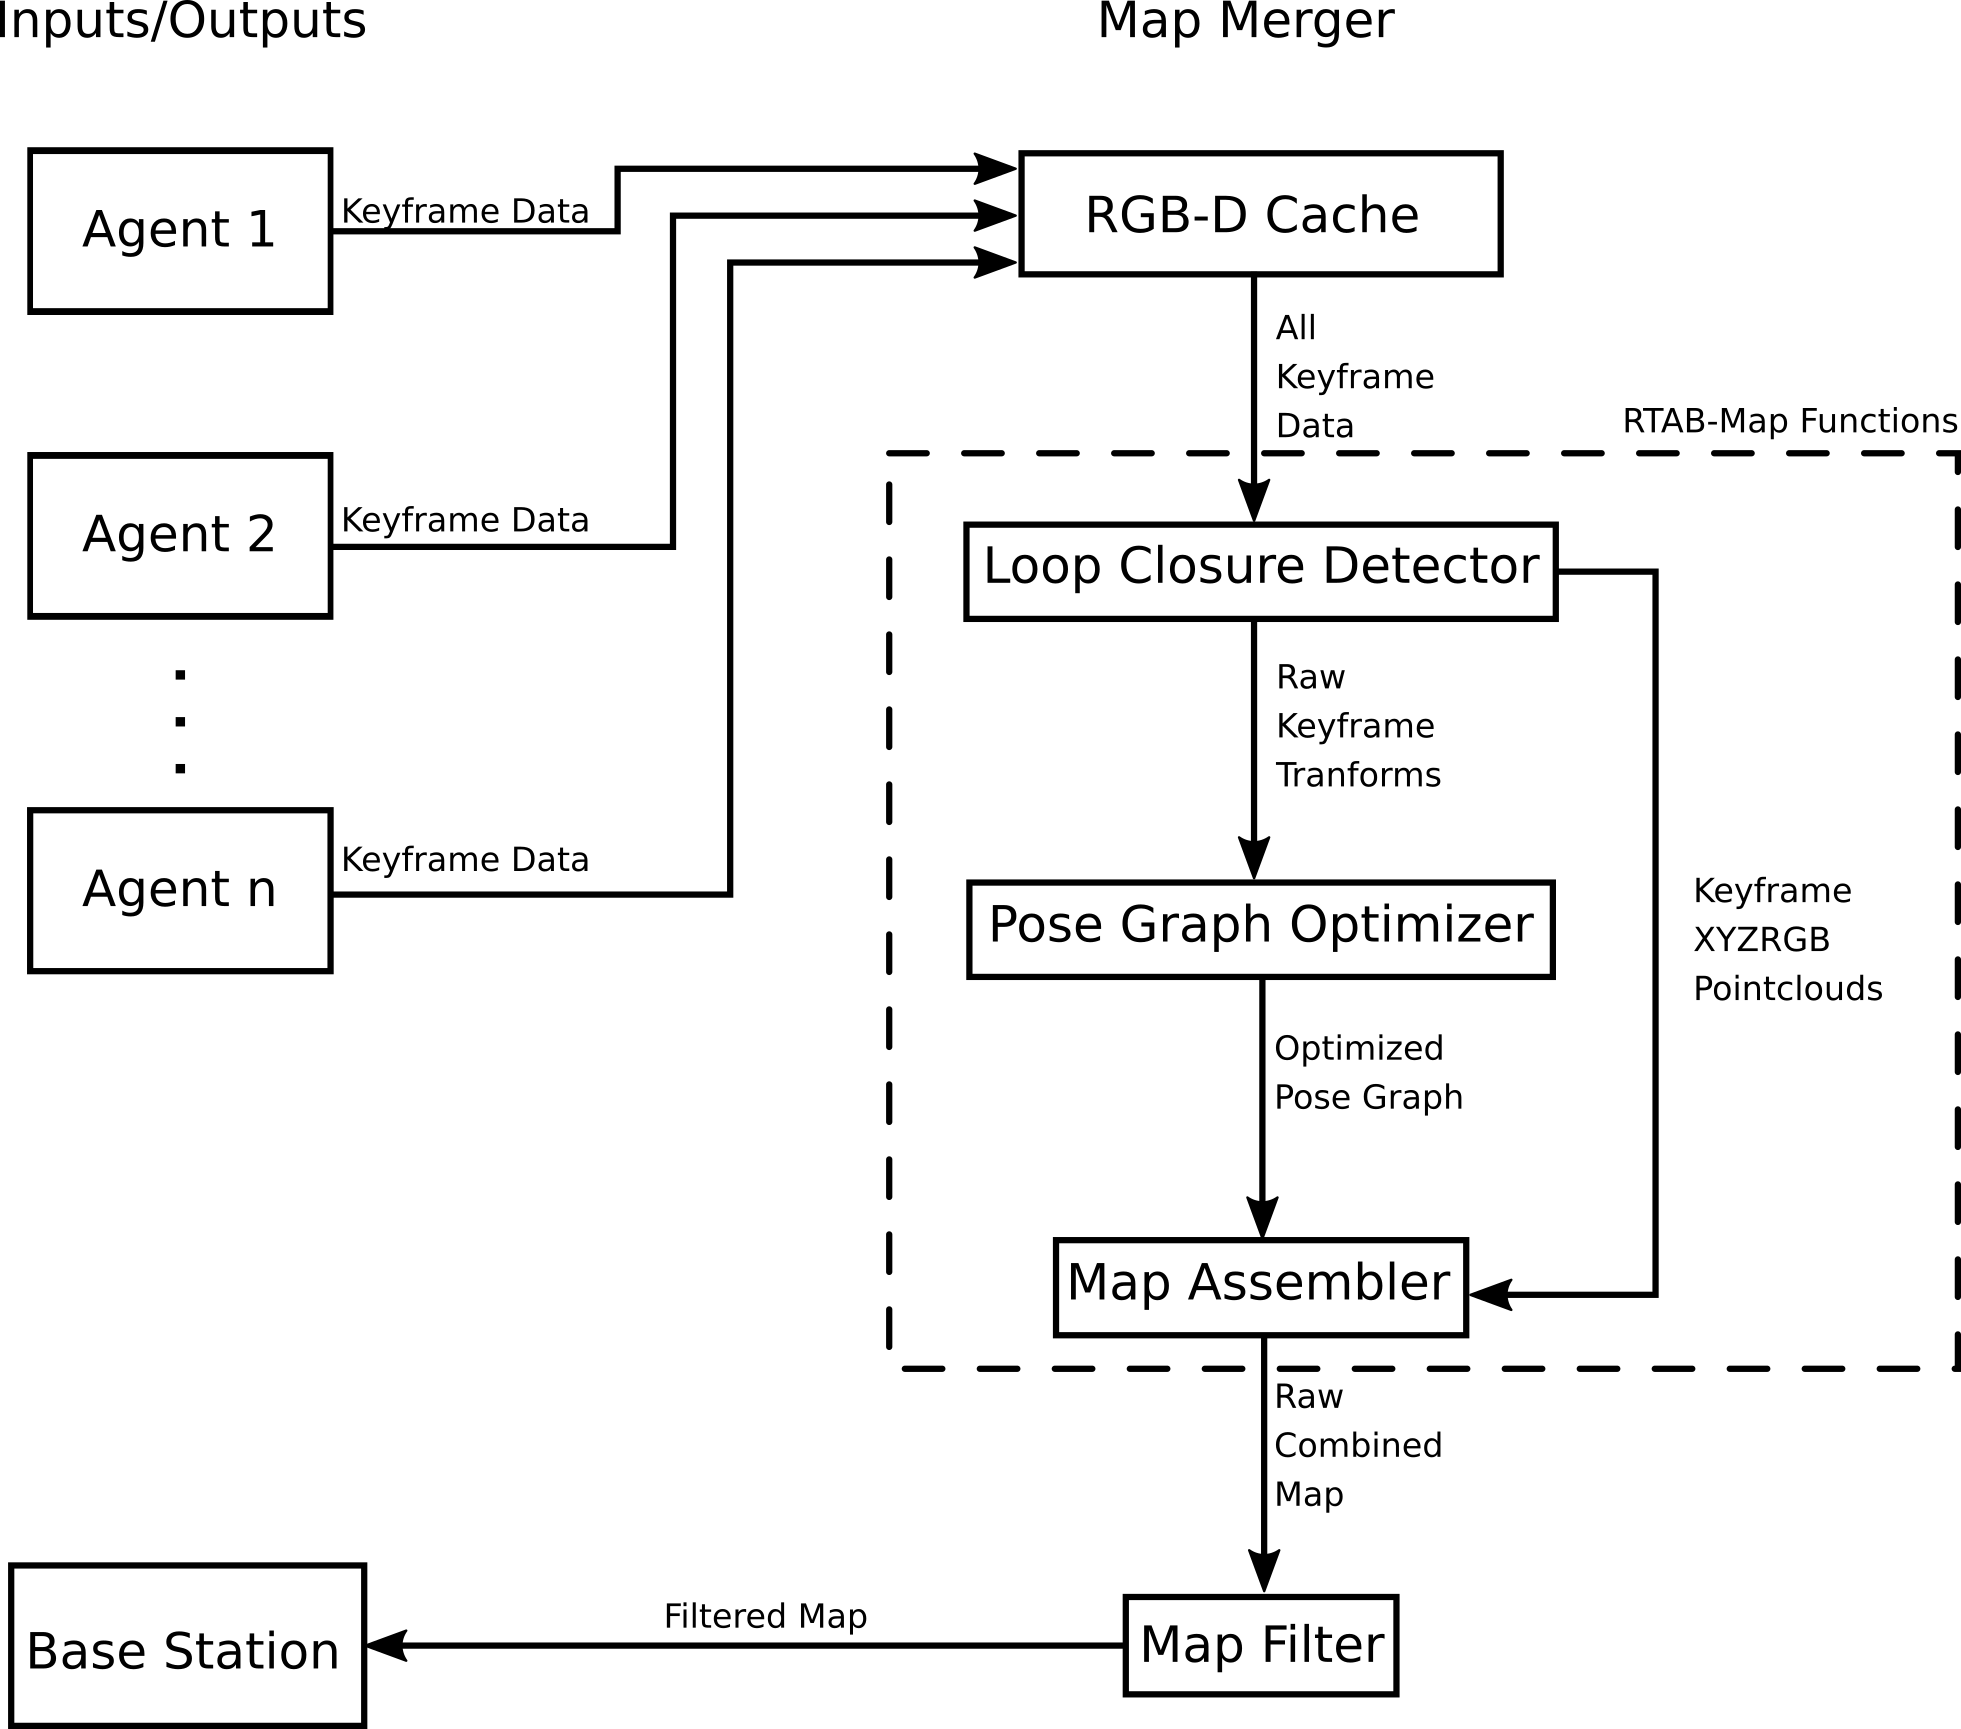
\includegraphics[width=0.7\linewidth]{map_merger_network}
\caption{The network diagram for the multi-agent map merging node proposed in this section.}
\label{fig:map_merge}
\end{figure*}

Once the database has been initialized, the maps are periodically merged using functions from an instance of RTAB-Map running on the base station computer similarly to how individual maps are generated for each UAV as described in \cite{Labbe2011}\cite{Labbe2013}\cite{Labbe2019}. The first step is to search for loop closures in the image features from each keyframe using a bag-of-words approach. Rather than only look for loop closures from the keyframes of a single agent, this process looks for loop closures from all keyframes from all agents. Each time a new loop closure is found, a new edge is added to combined map graph with an estimated transformation between keyframes. After finding all loop closures with the current dataset, the graph is optimized using the pose graph optimizer built into RTAB-Map, the optimized pose graph is then sent to the map assembler along with the XYZRGB pointcloud from each keyframe where the pointclouds are combined according to the optimized graph edges. This generates a single map with all keyframes that can be connected into a single graph. This map is then processed to remove some noise and filter out the ceiling to make the map more understandable to the operator.
%%%%%%%%%%%%%%%%%%%%%%%%%%%%%%%%%%%%%%%%%%%%%%%%%%%%%%%%%%%%%%%%%%%%%%%%%%%%%%%%
\section{Results and Discussion}\label{results}

\subsection{Simulation}

\begin{figure}
\centering
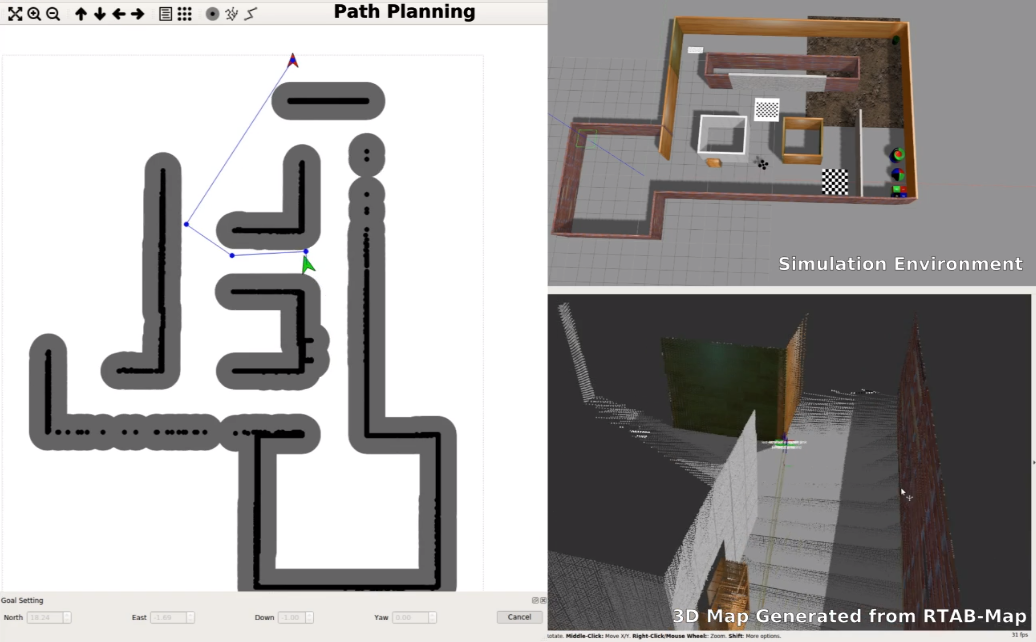
\includegraphics[width=1.0\linewidth]{sim_setup}
\caption{Setup used for the simulation results}
\label{fig:sim_setup}
\end{figure}

\subsection{Hardware}

\begin{figure*}
\centering
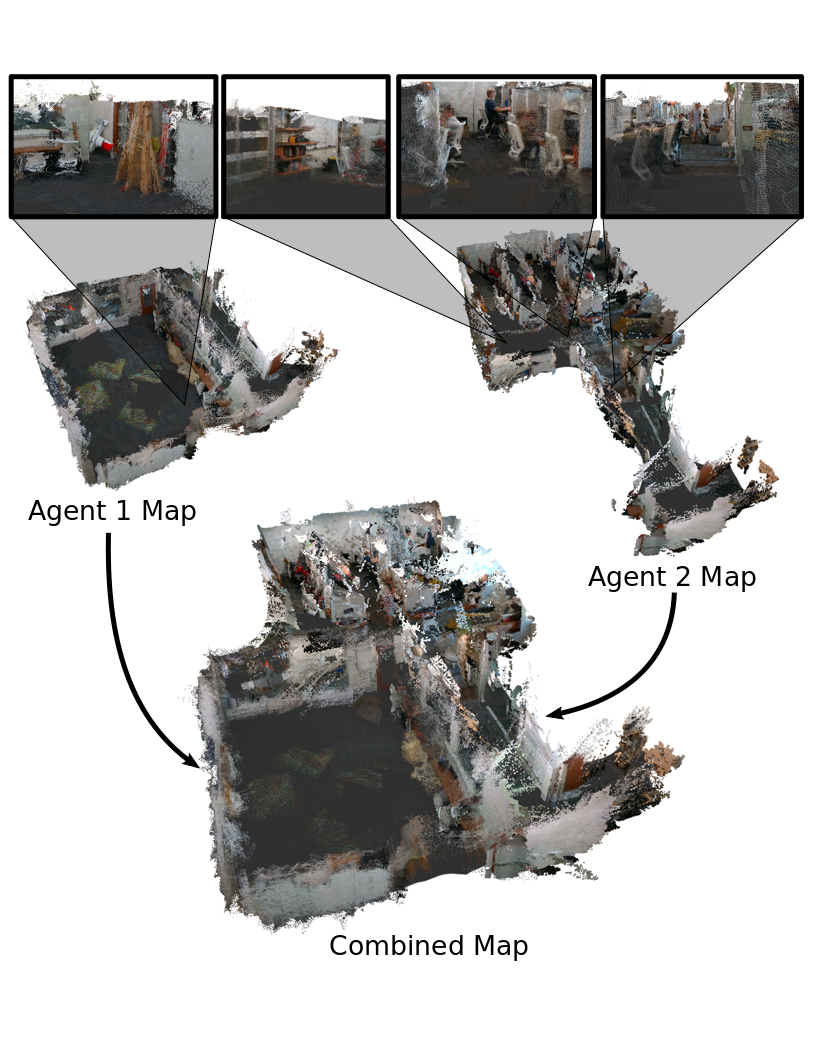
\includegraphics[width=0.9\linewidth]{lab_map.png}
\caption{Example of hardware results of merging maps from two agents into a single map in a cluttered environment. Above the individual agent maps are examples of the detail in the pointclouds when zooming in.}
\label{fig:lab_map}
\end{figure*}

\begin{figure*}
\centering
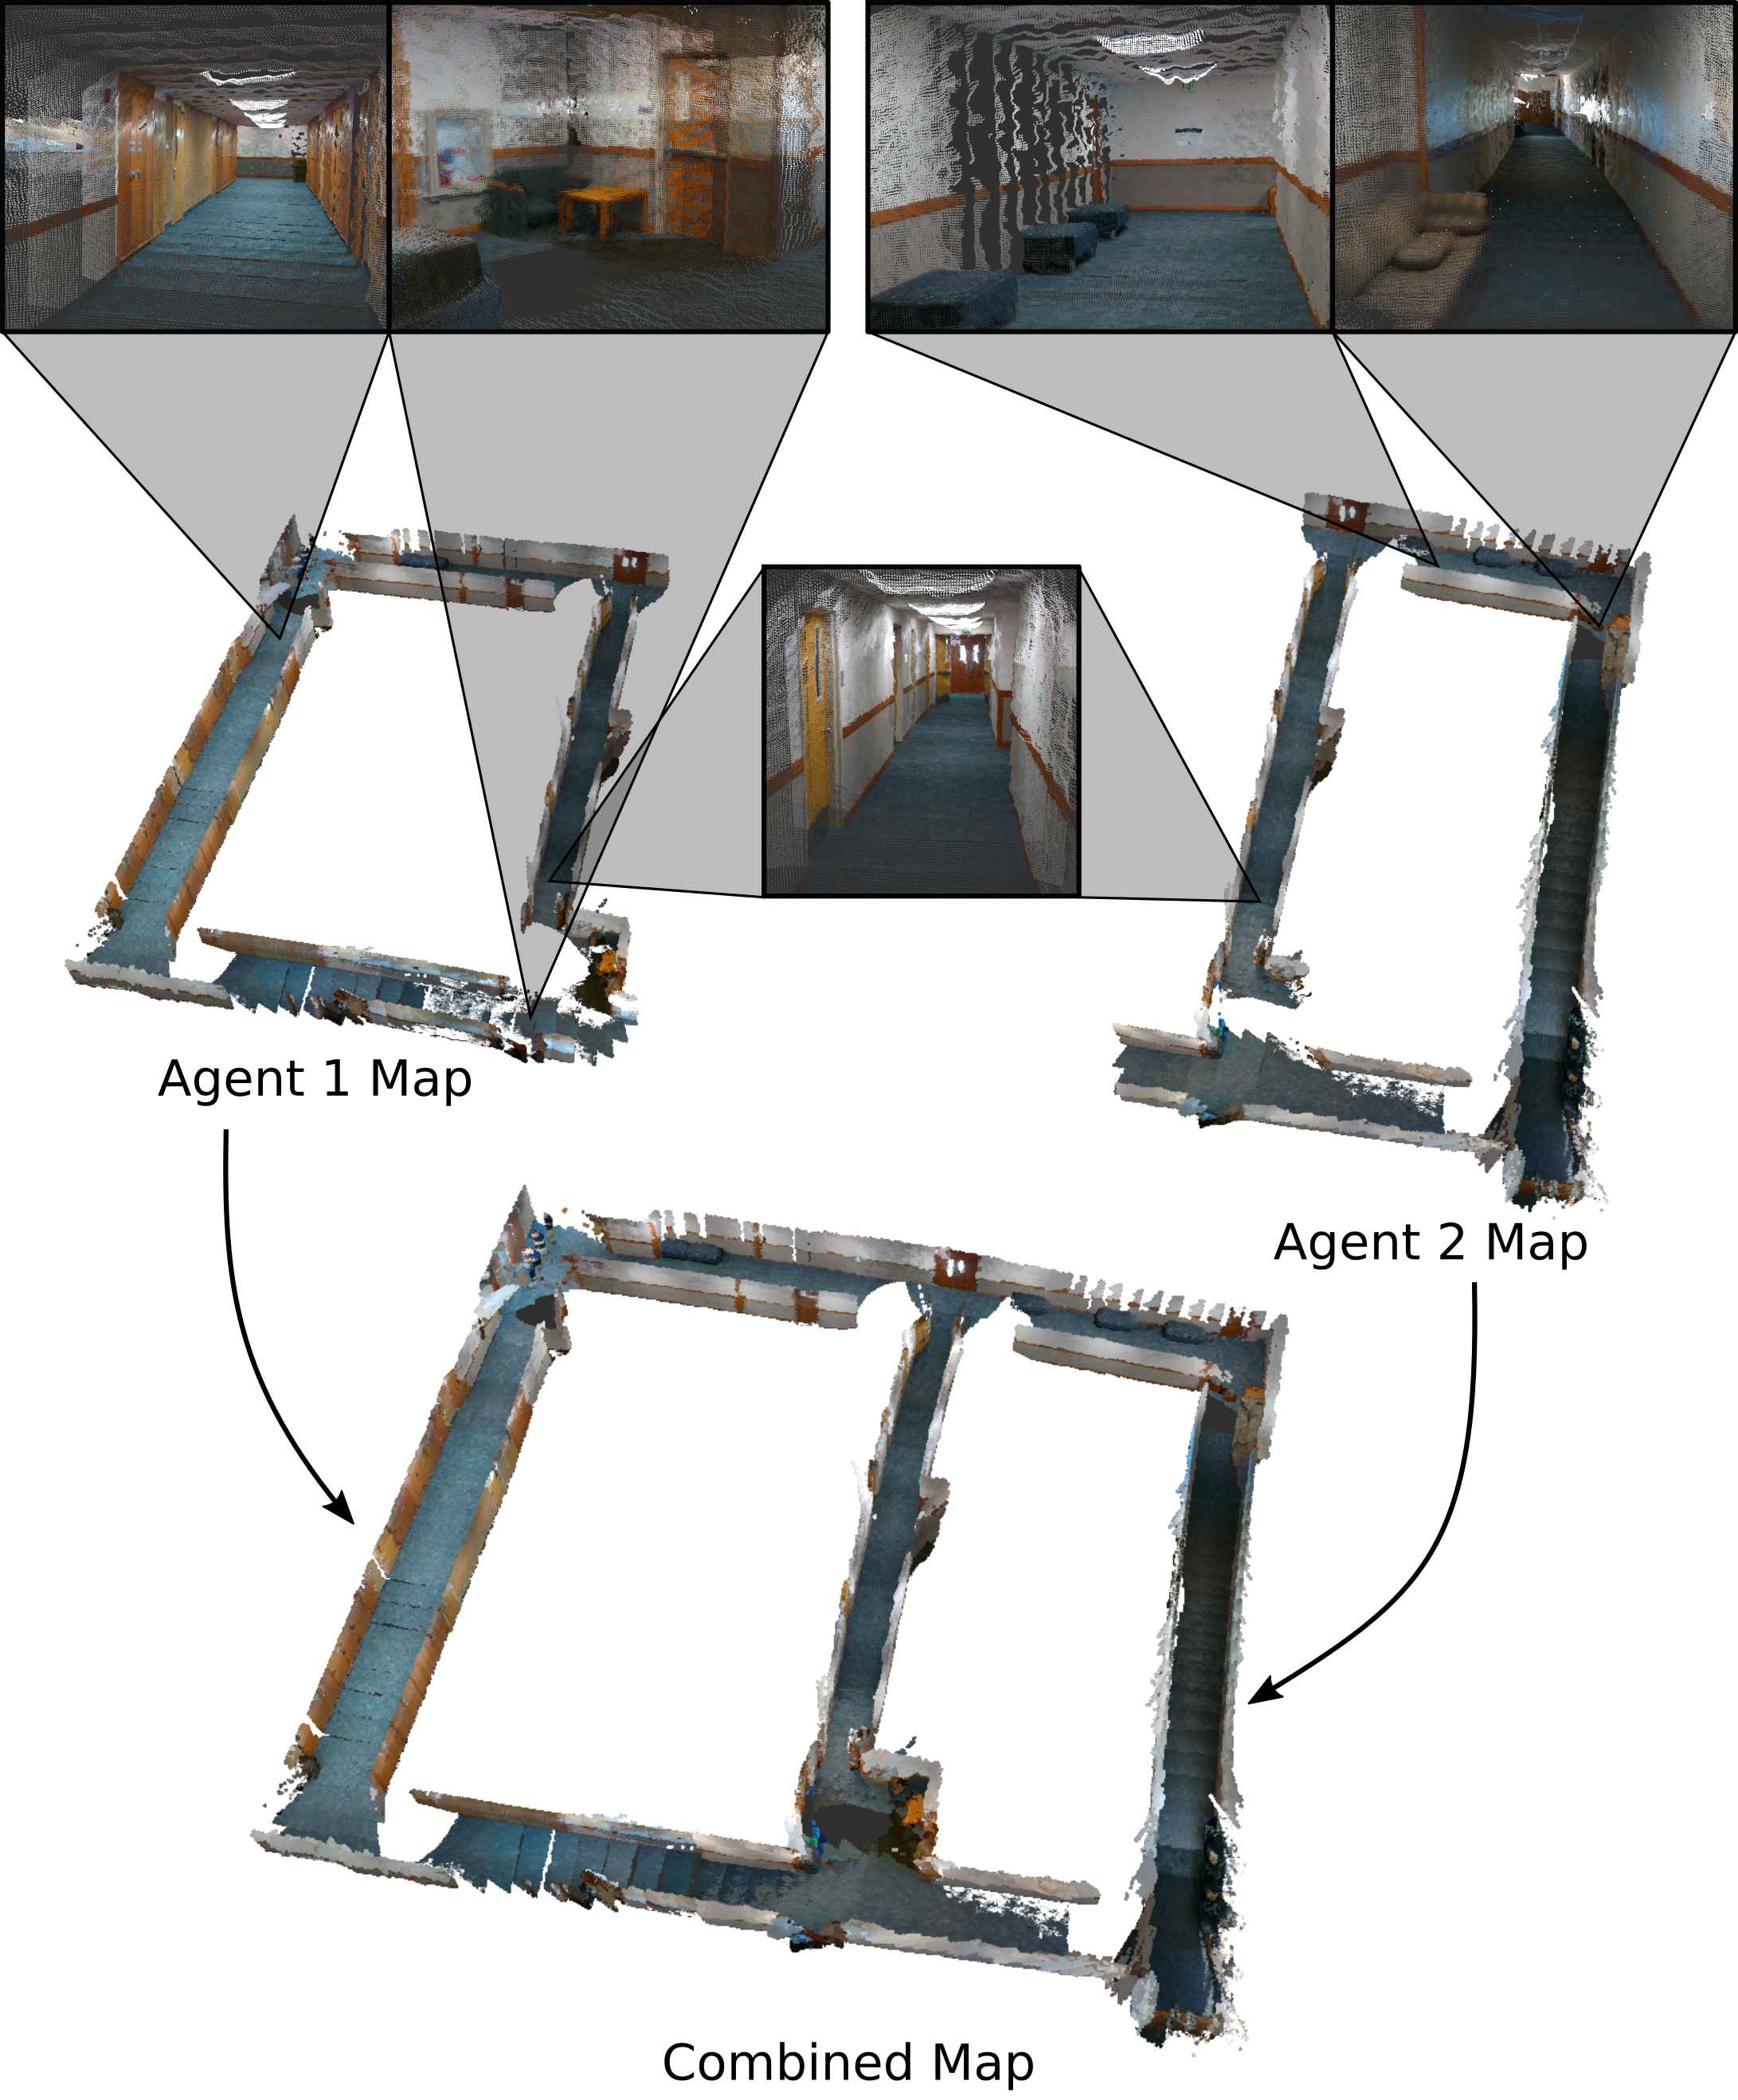
\includegraphics[width=0.9\linewidth]{wilk3_map.png}
\caption{Example of hardware results of merging maps from two agents into a single map in a simpler hallway environment. Above the individual agent maps are examples of the detail in the pointclouds when zooming in.}
\label{fig:wilk3_map}
\end{figure*}
%%%%%%%%%%%%%%%%%%%%%%%%%%%%%%%%%%%%%%%%%%%%%%%%%%%%%%%%%%%%%%%%%%%%%%%%%%%%%%%%
\section{Conclusions}\label{conclusions}


%%%%%%%%%%%%%%%%%%%%%%%%%%%%%%%%%%%%%%%%%%%%%%%%%%%%%%%%%%%%%%%%%%%%%%%%%%%%%%%%

\bibliographystyle{IEEEtran} % We choose the "plain" reference style
\bibliography{mapping_paper_2019}

\end{document}
